\cotefile{43}
\scanpage{195}
% archive sheet number: 194
% source line 1
\uline{Catégories abéliennes}

% source lines 2--15
Soit $\unsure{\underline{C}|\underline{\mathcal{C}}}$ une catégorie abélienne où tous les objets sont de longueur finie. Alors $\operatorname{Ind}\underline{C}$ [catégorie des foncteurs contravariants exacts à gauche de $\underline{C}$ dans \deleted{\unsure{Ens}} $(\mathrm{Ab})$] est une \uline{catégorie abélienne} à \uline{limites inductives exactes}, à générateurs de longueur finie [nous dirons : \uline{loc. de longueur finie}] dont $\underline{C}$ est la sous-catégorie des objets de longueur finie. Il y a ainsi \unsure{essentiellement} correspondance biunivoque entre catégories abéliennes à objets de longueur finie, et catégories abéliennes à limites inductives exactes à générateurs de longueur finie.

% source lines 16--21; insertion above line 16
Soit $\underline{C}$ une catégorie abélienne\inserted{à limites inductives exactes}, $X\in\underline{C}$, le \uline{socle} de $X$ est la \deleted{\illegible{1}} somme des sous-objets simples de $X$, soit $F_0(X)$. On désigne par $F_1(X)$ l'image inverse du socle de $X/X_0$ etc, et on \unsure{trouve} ainsi une filtration croissante. \deleted{\unsure{Si} $\underline{C}$ \unsure{est}}

\scanpage{196}
% archive sheet number: 195
% source lines 1--5
Cette \uline{filtration est fonctorielle} $\unsure{\underline{C}|\underline{\mathcal{C}}}$ loc. de longueur finie $\Leftrightarrow$ tout $X$ est le $\sup$ des $F_i(X)$. Soit en général $\Phi_0(X)=\operatorname{Sup}F_i(X)$, c'est le plus grand sous-objet de $X$ qui est ``de dim de Krull 0''.
% source insertion after line 5, continued between the lines and in the left margin
\inserted{C'est le noyau de $X\longrightarrow X_{C_0}$ (localisé par $C_0$) où $X_{C_0}$ est le \unsure{localisé} de $X$ pour la \unsure{ss-catégorie} $C_0$ de $C$ des objets de dim de Krull 0}
% slanted continuation of the insertion: de dim de Krull 0
% source lines 6--11
\unsure{On} introduit de \unsure{\deleted{même}|même} $\Phi_1(X)$ comme l'image inverse de $\Phi_0(X_{C_0}\deleted{\unsure{/\Phi_0(X)}})$\inserted{ou comme $\operatorname{Ker}(X\longrightarrow X_{C_1})$}. On en \unsure{trouve} encore une \uline{filtration} \uline{fonctorielle} $(\Phi_i(X))_i$. Dire que $\underline{C}$ est de dim de Krull $\leq n$ signifie que $\Phi_n(X)=X$ pour tout $X$.

\scanpage{197}
% archive sheet number: 196
% source top-left cancellation
\deleted{\unsure{Ab}}

% source top display, continued down the right edge
\[
\begin{aligned}
&\operatorname{ind}\bigl(\text{pro-(groupes alg. finis)}\ \deleted{\text{\unsure{artiniens}}}\inserted{\text{\unsure{noeth.}}}\bigr)\\
&\qquad=\operatorname{pro}\bigl(\text{Modules loc. de long. finie,}\ \text{\unsure{et} artiniens}\bigr)
\end{aligned}
\]
\begin{flushright}dont les Modules sur $A$.\end{flushright}

% source central diagram
\diagram{\begin{tikzcd}[ampersand replacement=\&,column sep=large,row sep=large]
\text{\uline{groupes formels raisonnables}}
 \arrow[r,Leftrightarrow,"\text{\unsure{contrav.}}"]
 \arrow[d,Leftrightarrow,"\text{\unsure{contrav.}}"]
 \& \begin{gathered}\text{Modules \uline{de type}}\\\text{fini sur }A\text{ tels}\\\text{que }M/FM\text{ soit}\\\text{de longueur finie}\end{gathered}\\
\text{pro-(\uline{groupes alg. finis}) \uline{raisonnables}}
 \arrow[ur,Leftrightarrow,"\text{cov.}"']
 \& \deleted{\text{\unsure{Mod}}}\arrow[u]
\end{tikzcd}}

% source lower half, isolated cancellations and computations
\[
\deleted{\unsure{A}}\qquad\deleted{\unsure{FV=p|FVE|FVE_{\!s}}}
\]
\[
\deleted{\unsure{w}}\ \sum_{-\infty}^{+\infty}\unsure{w_i|\omega_i}F^i+\sum_1^\infty w_jV^j
\]
\[
w_i\unsure{=|\to}0\quad\text{si}\quad i\longrightarrow\infty
\qquad /\quad W_\sigma[F][F^{-1}]
\]
% source lower-right crossed text block
% slanted
\margin{\deleted{\unsure{anneau} de \unsure{polynômes} \illegible{1} \unsure{relation} \unsure{non} \unsure{comm.}}}
\[
FV=p
\]
\[
\begin{aligned}
{\unsure{F|E}}^{-1}w_i&=\sigma^{-1}(w_i)F^{-1} & V&=pF^{-1}\\
F^{-1}w_j&=\sigma^{-1}(w_j)F^{-1} & \deleted{\unsure{F^{-1}V^j=|F^{-1}V^3=}}&\deleted{\unsure{\cdot}}\\
w_i\unsure{f|F}&=\unsure{f|F}\sigma^{-1}(w_i) & \deleted{F^{-1}V}&
\end{aligned}
\]
% source right of the preceding formulas
\[
\deleted{\unsure{F|E}}\qquad FV=p
\]

\scanpage{198}
% archive sheet number: 197
% printed form: paper watermark; oriented sideways in the scan
EXTRA STRONG

\unsure{Commercial Bank}

\unsure{4713|E713}

% letterhead: printer's imprint, upside down in the lower right of the scan
\begin{flushright}
M. DUFOUR\\
VARITYPISTE\\
131, RUE LECOURBE\\
PARIS XV\textsuperscript{e}\\
$\blacksquare$\\
C. C. P. Paris 14.143-34\\
R. M. 140.029
\end{flushright}

\scanpage{199}
% archive sheet number: 198
% letterhead
\begin{flushleft}
M. DUFOUR\\
VARITYPISTE\\
131, RUE LECOURBE\\
PARIS XV\textsuperscript{e}\\
$\blacksquare$\\
C. C. P. Paris 14.143-34\\
R. M. 140.029
\end{flushleft}
% source top definition
\[
W_{n,k}=\operatorname{Ker}(W_n\overset{F^k}{\unsure{-|\longrightarrow}}W_n)
\]
\diagram{\begin{tikzcd}[ampersand replacement=\&]
W_{n,k}\arrow[r,"i"]\arrow[d,"V"']\&W_{n,k'}\arrow[d]\&k'\geq k\\
W_{n+1,k}\arrow[r,"i"]\&W
\end{tikzcd}}
% source middle left and middle right
\[
\overline{W}_n=\bigcup_k W_{n,k}
\]
\diagram{\begin{tikzcd}[ampersand replacement=\&]
W_{1,k}\arrow[r,"V"]\&W_{2,k}\arrow[r]\&W_{3,k}\arrow[r]\&\cdots
\end{tikzcd}}
% slanted; the marginal question is enclosed in an oval
\margin{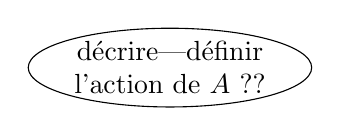
\begin{tikzpicture}\draw (0,0) ellipse (1.8cm and 0.5cm);\node[align=center] at (0,0) {\unsure{décrire|définir}\\\unsure{l'action} de $A$ ??};\end{tikzpicture}}
\diagram{\begin{tikzcd}[ampersand replacement=\&]
\overline{W}_1\arrow[r]\&\overline{W}_2\arrow[r]\&\cdots\&\overline{W}_n\arrow[r]\&\cdots
\end{tikzcd}}
\[
\unsure{U|\mathcal{U}}=\varinjlim_i\overline{W}_i
\]
% source lower centre; isolated V immediately below the F map
\[
F:U\longrightarrow U\qquad\overline{W}_1\qquad\underline{U}\subset V
\]
\[
V
\]
% source lower-left bracketed calculation
\diagram{\(\left\lfloor\begin{gathered}
\begin{tikzcd}[ampersand replacement=\&]
W_4\arrow[r,dash,"V_{4,5}"]\&W_5\arrow[r,dash]\&\unsure{w_1|W_1}\\
w\arrow[u]\arrow[r,"V"]\&W\arrow[u]\arrow[r,dash]\&w_1
\end{tikzcd}\\
V(\unsure{w|\omega})\qquad w\in W_\infty\\
\deleted{\unsure{w}}\ w\unsure{\xi|\zeta}\\
V(wx)=\sigma^{-1}(w)V(x)
\end{gathered}\right.\)}
% source right, above the inclusion chain
\[
w_1\qquad\sigma^{-1}(w)_2\qquad\sigma^{-2}(w)_2\qquad\sigma^{-3}(w)_3
\]
\[
\overline{W}_1\subset\overline{W}_2\subset\overline{W}_3\subset\overline{W}_4\subset\cdots
\qquad\underset{R}{\longleftarrow}
\]
% source below the large left bracket
\diagram{\begin{tikzcd}[ampersand replacement=\&]
w_3\&w_4\&\overline{G}_a\\
W_3\arrow[u,"\sigma^{-2}(w)"]\arrow[r]\&W_{\unsure{4|9}}\arrow[u,"\sigma^{-3}(w)"']
\end{tikzcd}}
% source bottom right, struck relation and boxed relations
\[
\deleted{FR=RF=p}
\]
\[
\boxed{\begin{gathered}FV=VF=p\\F^nU=0\\p^nU=0\end{gathered}}
\]

\scanpage{200}
% archive sheet number: 199
% source top-left cancelled beginning
\[
\deleted{\unsure{w+}}\qquad\deleted{\unsure{\sigma(w)}F+\sum}
\]
% source top-right, enclosed defining relations
\[
A=W_\infty[[F,V]]\qquad
\left\{\begin{aligned}
FV&=VF=p\\
F\unsure{w|\omega}&=\sigma(w)F\\
wV&=\deleted{\unsure{\sigma(w)}}V\sigma(w)
\end{aligned}\right.
\]
% source upper-left computations, lines 2--6
\[
w+\sum_{\unsure{1|0}}^\infty w'_iF^i+\sum_1^\infty w''_j\deleted{\unsure{F^i}}V^j
\]
\[
\deleted{\sum_0^\infty\sigma(w_i)F^{i+1}+\sum_0^\infty\sigma(\unsure{w'_i|w_i})F^{i+1}V}
\]
\[
\sum_0^\infty\sigma^{-1}(\unsure{w_i|w'_i})VF^i+\sum_0^\infty\sigma^{-1}(w'_i)VF^iV
\]
\[
\begin{aligned}
&w+\sum_1^\infty w'_iF^i+\sum_1^\infty w''_jV^j\\
&p\sigma(w''_{\unsure{1|0}})+\left(\sigma(w)F+\sum_2^\infty\sigma(w'_{i-1})F^{i\deleted{\unsure{+1}}}\right)+\left(\sum_1^\infty p\sigma(w''_{j+1})V^{j\deleted{\unsure{+1}}}\right)\\
&p\sigma^{-1}(w'_{\unsure{i|1}})+\left(\sum_1^\infty p\sigma^{-1}(w'_{i+1})F^i\right)+\left(\sigma^{-1}(w)V+\sum_1^\infty\sigma^{-1}(w''_j)V^{j+1}\right)
\end{aligned}
\]
% source middle, isolated C and right-hand note
\[
\unsure{C|\mathcal{C}}
\]
\margin{\uline{\unsure{hyperalgèbres}} \deleted{\illegible{1}} \uline{\unsure{artiniennes|artiniens}}}
\par\noindent\rule{\linewidth}{0.4pt}\par
% source below horizontal divider
\[
\operatorname{pro}\bigl(\text{\uline{groupes formels \inserted{abéliens} sur $k$}}\bigr)
\]
\uline{groupes formels artiniens sur} $k$

% source bottom comparison diagram
\diagram{\begin{tikzcd}[ampersand replacement=\&,column sep=large,row sep=large]
\begin{gathered}\text{grp alg. commutatif fini}\\\text{(d'Hyperalgèbre }U\text{)}\end{gathered}
 \arrow[r,Leftrightarrow]
 \&\begin{gathered}\text{Module de longueur finie}\\\text{sur }A\\\text{(savoir }\operatorname{Hom}(U,I)\text{)}\end{gathered}\\
\begin{gathered}\text{\deleted{\unsure{pro}}pro-(groupes alg. finis)}\quad\text{(noeth.)}\end{gathered}
 \arrow[r,Leftrightarrow]\arrow[d,Leftrightarrow,"\text{par dualité}"]
 \&\begin{gathered}\text{Modules loc. de longueur}\\\text{finie sur }A\ \text{(art)}\end{gathered}\\
\text{``groupes formels''}\quad\text{(art.)}
 \arrow[r,Leftrightarrow]
 \&\begin{gathered}\text{Modules de \deleted{\unsure{longueur}}}\\\deleted{\text{(noeth.)}}\\\equiv\\\text{(noeth. i.e. mod. de}\\\text{type fini sur }A\text{.)}\end{gathered}
\end{tikzcd}}
% letterhead: printed imprint upside down, overlapped by the bottom-right handwriting
\begin{flushright}
M. DUFOUR\\
VARITYPISTE\\
131, RUE LECOURBE\\
PARIS XV\textsuperscript{e}\\
$\blacksquare$\\
C. C. P. Paris 14.143-34\\
R. M. 140.029
\end{flushright}

% printed form: faint paper watermark, sideways beneath the mathematical notes
EXTRA STRONG

\unsure{Commercial Bank}

\scanpage{201}
% archive sheet number: 200
% source upper diagram
\diagram{\begin{tikzcd}[ampersand replacement=\&,column sep=large,row sep=large]
\text{groupes formels raisonnables \uline{mod \unsure{isogènie|isogénie|isogenie}}}
 \arrow[d,Leftrightarrow,"\text{\unsure{contr.}}"]
 \arrow[dr,Leftrightarrow,"\text{\unsure{anti}}"]\&\\
\begin{gathered}\text{\uline{progroupes alg. finis raisonnables}}\\\text{\uline{mod \deleted{\unsure{isog.}} groupes alg. finis}}\end{gathered}
 \arrow[r,Leftrightarrow,"\text{cov.}"]
 \&\begin{gathered}\text{\uline{Modules}}\\\text{\uline{de torsion}}\\\deleted{\text{\unsure{sur}}}\\\text{\uline{de type fini}}\\A_F\\=\text{\uline{modules}}\\\text{\uline{de long. finie}}\\\text{\uline{sur $A_F$}}\end{gathered}
\end{tikzcd}}
% source centre-left fork
\diagram{\begin{tikzcd}[ampersand replacement=\&]
\&\&W_\sigma[F,V]\\
\underline{W}\arrow[r]\&\underline{A}_F=\unsure{\mathcal{A}|\mathscr{A}}\arrow[ur,equal]\arrow[dr,dash]\&\\
\&\&\deleted{\unsure{\sigma}}W_n
\end{tikzcd}}
\[
F\ V
\]
% source lower boxed text
\noindent\fbox{\begin{minipage}{0.92\linewidth}
Modules de type fini $M$ sur $W$

Muni d'une application \inserted{additive \uline{bijective}} $F:M-M$ et d'une application additive : $V:M-M$
\[
\text{tels que}\quad\left\{\begin{aligned}
F(\unsure{w|\omega}x)&=F(w)F(x)\\
V(wx)&=F^{-1}(w)V(x)
\end{aligned}\right.
\]
\end{minipage}}
% source below the box, left
\[
\unsure{R|\mathscr{R}}\quad W
\]
% letterhead: upside down in lower right
\begin{flushright}
M. DUFOUR\\
VARITYPISTE\\
131, RUE LECOURBE\\
PARIS XV\textsuperscript{e}\\
$\blacksquare$\\
C. C. P. Paris 14.143-34\\
R. M. 140.029
\end{flushright}

% printed form: faint sideways watermark beneath the notes
\unsure{EXTRA STRONG}

\unsure{Commercial Bank}

\scanpage{202}
% archive sheet number: 201
% source lines 1--2
$\unsure{m|\mathfrak{m}}/m^2$ dual de $P(U)$ primitifs, \deleted{\unsure{espace de}} \unsure{de dim} finie \unsure{sur}
\[
=\unsure{\text{tange}|\text{tang.}|\text{tué}}\ \text{par le \unsure{noyau} de }F.
\]
% source lines 3--10
s'il est de dim finie, le \uline{socle} est fini, donc on a un objet \uline{artinien} [N.B. l'injectif \inserted{indécomp.} de la catégorie des \unsure{bigèbres|algèbres} de Dieudonné est artinien \unsure{...}], donc on a un module \deleted{\unsure{noeth.}} de Chevalley artinien = module de type. fini sur $A$. De plus, la condition est que $M/FM$ est de dim finie sur $k$ i.e. \uline{de longueur finie}.

% source centre-right enclosed conclusion
\noindent\fbox{\begin{minipage}{0.55\linewidth}
Ceci indique que le module $M$ est un module de torsion
\end{minipage}}
% source centre-left category diagram and its two exterior braces
\diagram{\begin{tikzcd}[ampersand replacement=\&,column sep=small]
A_F\ \left\{\vphantom{\begin{matrix}C\\C_1\\C_F\end{matrix}}\right.\&\&\unsure{C|\mathcal{C}}\&\&\left.\vphantom{\begin{matrix}C\\C_1\\C'_F\end{matrix}}\right\}\ A_S\&\text{\textcircled{\small $S=A-F$}}\\
\&\&C_1\arrow[u]\&\\
\&C_F\arrow[ur]\&\&C'_F\arrow[ul]\\
\&\&C_0\arrow[ul]\arrow[ur]\arrow[d,dash]\\
\&\&0
\end{tikzcd}}
% source lower-left note beside C_F/C_0
\margin{\unsure{cat. primaire} \deleted{\unsure{d'objets}} \unsure{engendrée} dans $C/C_0$ par l'objet $(A/FA)_{C_0}$ \uline{simple} $\unsure{\omega|w}$}
% source lower-middle note, linked by a brace to C'_F and C_0
\unsure{cat. primaire gauche}. \unsure{engendrée} dans $C_1/C_0$ par les autres objets simples de $C_1/C_0$, sur $F$ est \deleted{bijectif}\inserted{surjectif} dans l'objet mod $C_0$
\[
C_1/C_0\simeq C_F/C_0\times C'_F/C_0
\]
% source small drawing in the right margin; two crossing curved strokes
\figure{\begin{tikzpicture}[scale=0.7]
\draw[gray] (0,0) .. controls (0.8,1.1) and (1.6,1.8) .. (3,2);
\draw (1,2.1) .. controls (0.95,1.2) and (1.1,1) .. (1.65,0.55);
\fill (1.05,1.25) circle (1.3pt);
\end{tikzpicture}}
% source right-hand notes, over the printer's imprint
\margin{\uline{limites projectives d'objets artiniens}}
% source bottom-left bracketed fragments; the manuscript leaves the opening brackets unclosed
[objet \deleted{\unsure{simple}} \unsure{engendré} par $A/FA$

[objet \deleted{\unsure{noeth.}} \unsure{engendré;} par $A/VA$

\uline{\unsure{deux} objets \deleted{\unsure{non}} simples}
\[
\deleted{\unsure{A}}\unsure{F_2|F^2}
\]
\margin{\uline{limites inductives d'objets noethériens}}
% letterhead: upside down in lower right, overlapped by notes
\begin{flushright}
M. DUFOUR\\
VARITYPISTE\\
131, RUE LECOURBE\\
PARIS XV\textsuperscript{e}\\
$\blacksquare$\\
C. C. P. Paris 14.143-34\\
R. M. 140.029
\end{flushright}

\scanpage{203}
% archive sheet number: 202
% source upper-right title, two manuscript lines
\begin{flushright}
\unsure{Accouplements|Accouplement} de $\unsure{\Phi|\mathscr{F}|F}$\\
Tate - Lang
\end{flushright}

\scanpage{204}
% archive sheet number: 203
% source upper-right heading
\begin{flushright}\uline{Accouplements de Tate}\\(schéma préliminaire)\end{flushright}
% source lines 1--2 left
$A$ schéma abélien sur $S$

$P$ fibré principal homogène sous $A$

% source lines 3--4
$\underline{\operatorname{Pic}}^{\unsure{*|\tau}}_{\deleted{\unsure{*}}A/S}$ schéma en groupes, contenant le schéma abélien $\underline{\operatorname{Pic}}^0_{A/S}=A'$ schéma \uline{dual} de $A$

% source lines 5--7
$A$ opère sur lui-même par automorphismes donc opère sur $\operatorname{Pic}^*_{A/S}$ et par suite sur $A'$, et opère \uline{trivialement} sur $A'=\underline{\operatorname{Pic}}^0_{A/S}$ et $\underline{\operatorname{Pic}}^*_{A/S}/\underline{\operatorname{Pic}}^0_{A/S}=\mathrm{N.S.}_{A/S}$
\[
\left[\ \text{donc}\quad A\times\underbrace{\underline{\operatorname{Pic}}^*_{A/S}/\underline{\operatorname{Pic}}^0_{A/S}}_{\text{Néron--Séveri}}\longrightarrow\underset{\substack{\Vert\\A'}}{\underline{\operatorname{Pic}}^0_{A/S}}\ \right]
\]
% source left marginal calculation, with labels pointing up to the terms
\margin{\begin{tikzcd}[ampersand replacement=\&,column sep=tiny,row sep=small]
\unsure{gx|g*x}\&x+\&\lambda\cdot\&\overline{x}\\
\&\operatorname{Pic}^*_{A/S}(T)\arrow[u]\&A(T)\arrow[u]\&\mathrm{N.S.}(T)\arrow[u]
\end{tikzcd}}
% source lines 9--17
Considérons $\underline{\operatorname{Pic}}^*_{P/S}$, il a une ``\uline{composante connexe} \inserted{\uline{neutre}}'' $\underline{\operatorname{Pic}}^0_{P/S}$, \uline{qui est can. isom. à} $\operatorname{Pic}^0_{A/S}=A'$ [car $A$ y opère trivialement] -- car $\underline{\operatorname{Pic}}^*_{P/S}$ est \uline{associé} à $P$ et à $\operatorname{Pic}^*_{A/S}$ sur lequel $A$ opère de la façon naturelle. [il est \unsure{extension} de $\mathrm{NS}_{A/S}$ par $\underline{\operatorname{Pic}}^0_{A/S}=A'$, donc il lui correspond \margin{\deleted{$\unsure{\xi|\varepsilon|\lambda}$}} un élément de $\operatorname{Ext}^1_S(\mathrm{N.S.}_{A/S},A')$, donc pour \unsure{tte} \deleted{\unsure{hom|une}} \deleted{\unsure{élément|classe}}\inserted{\unsure{section}} de $\mathrm{N.S.}_{A/S}$ une classe de $H^1(S,A')$, \unsure{qui s'interprète} \unsure{évidemment}\ldots]

% source final two lines, continued on next scan
Si alors on a une section de $A'$, l'obstruction à l'obtenir à partir d'une

\scanpage{205}
% archive sheet number: 204
% top, continuation from scan 204; the first deleted word stands above the second
classe de faisceaux inversibles \deleted{\unsure{de}} \deleted{\unsure{locaux}} sur $S$ est dans le Groupe de Brauer $H^2(S,\unsure{\mathbb G_m|G_m})$ [\unsure{se rappeler|se rappelle} que
\[
\begin{aligned}
H^*(S,\mathbb G_m)&\underset{p}{\Longleftarrow} H^p(\unsure{B|S},\underline H^q_{\unsure{\mathrm{local}|\mathrm{loc}}}(\mathbb G_m))\quad\text{donc}\\
H^n(S,\mathbb G_m)&\unsure{\longrightarrow|-} H^0(S,\underline H^n_{\unsure{\mathrm{loc}|\mathrm{local}}}(\mathbb G_m))\quad\cdots
\end{aligned}
\]
]. On obtient ainsi l'\uline{accouplement de Tate}
\[
\boxed{H^1(S,A)\times H^0(S,A')\longrightarrow H^2(S,\mathbb G_m)}
\]

% middle
\unsure{Ceci} d'ailleurs se \unsure{précise}. (\unsure{Supposons p.ex.} que $S'\longrightarrow S$ est fid plat) \unsure{on a} des accouplements
\[
H^1(S'/S,A)\times H^0(S,A')\longrightarrow H^2(S'/S,\mathbb G_m).
\]

% bottom
Il semble, quand $S'$ est \uline{fini} sur $S$, de sorte que les $\widehat H^i(S'/S,A)$ sont définis, qu'on puisse définir \unsure{même} des accouplements
\[
\widehat H^i(S'/S,A)\times\widehat H^{1-i}(S'/S,A')\longrightarrow H^2(S'/S,\mathbb G_m)
\]
qu'il faudrait comprendre \ldots\ldots

\scanpage{206}
% archive sheet number: 205
% upper-right pencil heading
\begin{flushright}\fbox{\unsure{Symboles locaux}}\end{flushright}

$X$ courbe projective non singulière connexe \unsure{alg$/k$} \unsure{alg. clos}, $K=k(X)$.
Si $f,g\in k(X)^*$, $x\in X$, on définit
\[
\boxed{(f,g)_x=\frac{f^{\unsure{v_x(g)|\nu_x(g)}}}{g^{v_x(f)}}(x)(-1)^{v_x(f)v_x(g)}}
\]
% upper-middle, brace alongside (i)--(iv)
\unsure{On.}
\[
\left\{\begin{aligned}
\text{(i)}\quad&\text{On a une application bilinéaire}\quad K^*\times K^*\longrightarrow\unsure{K^*|k^*}\\
\text{(ii)}\quad&(f,g)_x=f(x)^{v_x(g)}=f\langle(g)_x\rangle\quad\text{si }f:X\longrightarrow\unsure{G_m|\mathbb G_m}\text{ déf. en }\unsure{x}\\
\text{(iii)}\quad&(f,g)_x=1\quad\text{si }g\text{ est une unité stricte}\inserted{\text{en }x}\text{ i.e. }g(x)=1\\
\text{(iv)}\quad&\prod_{x\in X}(f,g)_x=1
\end{aligned}\right.
\]
% left margin, alongside (iii)--(iv)
\margin{\unsure{c'est}, pour $f:X\longrightarrow G_m$ \unsure{donné}, un \uline{symbole} local en $g\in K^*$.}
\[
\text{(v)}\qquad(f,g)_x(g,f)_x=1
\]

% middle
On en déduit un accouplement
\[
\begin{aligned}
\unsure{\mathcal I|\mathcal J|I}(X)\times\mathcal I(X)&\longrightarrow k^*\\
(\vec f,\vec g)&=\prod_x(\unsure{\vec f_x|\bar f_x|f_x},g_x)_x
\end{aligned}
\]
\margin{$(\mathcal I(X),\text{\unsure{idèles}})$ \unsure{$v^\circ$|$\nu$}}
\unsure{On.}
\[
(\vec f,\vec g)=1\quad\left\{\begin{aligned}
&\text{si }\vec f\text{ est principal \uline{et} }\vec g\text{ principal}\ \deleted{\illegible{1}}\\
&\text{si }\vec f\text{ ou }\vec g\text{ est une unité stricte}
\end{aligned}\right.
\]

% lower third
En partic., $K^*$ et $UK^*$ sont orthogonaux, d'où des accouplements
\[
\boxed{K^*\times\underset{\substack{\text{classes d'}\\\deleted{\text{\unsure{diviseurs|équivalence}}}\inserted{\text{idèles}}\,=\,\mathcal I/\unsure{UK^*|K^*}}}{\deleted{\unsure{P|\mathcal P}}\unsure{C|\mathcal C}(X)}\longrightarrow k^*}
\]
qui induit un accouplement
% formula inserted in the space above the crossed-out pairing
\[
\unsure{\langle f,\vec g\rangle|(f,\vec g)}=f\langle D\rangle\prod_{x\in\operatorname{supp}f}g_x(x)^{-v_x(f)}
\]
% squeezed notation adjoining the right edge of the cancelled box
\margin{$\unsure{f\in k(X)|K(X)|C(X)}$}
si $(\vec g)$ et $(\vec f)$ sont premiers entre eux, $D$ étant la classe du diviseur de $\unsure{\vec f|\vec g}$.
\[
\deleted{\boxed{C(X)\times UK^*\longrightarrow k^*}}
\]
\deleted{\unsure{groupe d'idèles}}
\[
\boxed{\underbrace{K^*/k^*}_{\substack{\text{\unsure{diviseurs au|diviseurs des}}\\\text{\unsure{noyau d\textquotesingle Albanese}}}}\times\underset{\substack{\text{classes d'idèles}\\\text{de degré }0}}{\underline{C_0(X)}}\longrightarrow k^*}
\]

\scanpage{207}
% archive sheet number: 206
Voici la généralisation de Tate.

$X$ variété non singulière \unsure{alg$/k$ alg clos}, $K=k(X)$

$A:\unsure{A(V)|A(X)}$ var. d'Albanese, \inserted{hom $\unsure{\varphi|\phi}:X\longrightarrow A\deleted{\unsure{(X)|(V)}}$}, $\deleted{\unsure{P|\mathcal P}}$ $\widehat A$ variété de Picard.

Soient $\unsure{N|\mathcal N}$ le noyau d'Albanese : $N=\operatorname{Ker}(\unsure{\mathcal Z_0(X)|Z_0(X)}\longrightarrow A(X))$

\deleted{\unsure{On veut}}

$\unsure{\mathcal I|\mathcal J|I}$ le groupe des \unsure{données|classes} de répartitions
\[
\vec f=(f_x)_{x\in X}
\]
telles qu'il existe un diviseur $D$ sur $X$, avec $(f_x)_x=[D]_x$ pour tt $x$. On a une application
\[
C=\mathcal I/\deleted{\unsure{U}}K^*\longrightarrow\unsure{\mathcal P(X)|P(X)}
\]
(classes de diviseurs), soit $\deleted{\unsure{\mathcal I_0}}C_0$ l'\unsure{image} inverse de $\widehat A$; \unsure{donc on a} un hom surjectif
\[
C_0\longrightarrow\widehat A
\]
$\mathcal I_0$ est l'image réciproque de $C_0$ dans $\mathcal I$.
On veut définir un accouplement
\[
N\times C_0\longrightarrow k^*
\]
et pour ceci, on définit un accouplement
\[
N\times\mathcal I_0\longrightarrow k^*
\]
qui est trivial sur $N\times K^*$. Soit
\[
\unsure{z|\zeta}=\sum a_i\unsure{\tilde x_i|x_i|\xi_i}\in N,\qquad\deleted{\unsure{\deg z=0|\deg=0}}
\]
\inserted{$\xi\in C_0$,} $\vec f=(f_x)_{x\in X}\in\mathcal I_0$ un représentant de $\xi$ \inserted{tel que $\operatorname{div}(\vec f)$ ne rencontre pas $z$},
$D$ le diviseur défini par $\vec f$, $\deleted{\unsure{\xi}}\dot D$ son \unsure{image} dans $\widehat A$, et $z'\in\mathcal Z_0(\widehat A)$ \deleted{\unsure{avec}}, $\deg z'=0$, tel que $\dot D=S(z')$.
Soient $\Theta$ un diviseur canonique sur $\deleted{X}A\times\widehat A$ en \unsure{bonne position} pour $\varphi(z)\times\deleted{\unsure{\xi|z}}z'$, et considérons

\scanpage{208}
% archive sheet number: 207
% continuation from scan 207
\[
\lambda=\Theta\langle\deleted{\unsure{\varphi|\phi}}{\unsure{z|\zeta}}^{\deleted{\unsure{\xi|*}}},z'\rangle\deleted{\unsure{*}}
\]
qui est défini en notant que $\Theta\langle z\rangle$ est un \deleted{\unsure{diviseur|classe de}} diviseur sur $\widehat A$ qui est lin. équivalent à $0$, car sa classe est définie par $S\unsure{\varphi|\phi}(z)\in\unsure{\operatorname{Alban.}|\operatorname{Alb.}}$, qui est nul; donc on peut \deleted{prendre} trouver $g$ fonction sur $\widehat A$ telle que $(g)=\Theta\langle z\rangle$, et on prend
\[
\lambda=g\langle z'\rangle\qquad\text{(indépendant de }g\text{ car }\deg z'=0\text{)}
\]

D'autre part, on considère pour tout $x\in\deleted{X}\unsure{\operatorname{supp}z}$ le \deleted{\unsure{nb} $f_x(x)$} $f_{x_i}(x_i)^{a_i}$, et on pose
\[
\mu=\prod_i f_{x_i}(x_i)^{a_i}
\]
on pose alors
\[
\langle z,\xi\rangle=\lambda/\mu=\Theta\langle z,z'\rangle\,/\,\prod_i f_{x_i}(x_i)^{a_i}.
\]

Montrons que $\Theta\langle z,z'\rangle$ ne dépend que de $\dot D$ et $z$ : Si on change $\Theta$ en $\Theta+(h)$, ($h$ fonction sur $\unsure{\deleted{X}A|X}\times\widehat A$) \deleted{\unsure{donc et|donc}} on obtient
